\documentclass[14pt]{beamer}

\usepackage[utf8]{inputenc}
\usepackage[english]{babel}
\usepackage{amssymb}
\usepackage{pifont}

\newcommand{\xmark}{\ding{55}}

\setbeamercovered{transparent=40}
\beamertemplatenavigationsymbolsempty
\AtBeginSection[]{\subsection{}}
\usetheme{Frankfurt} 
\usecolortheme{frigatebird} 

\graphicspath{{./pictures/}}

\setbeamertemplate{title page}[default]
\setbeamertemplate{itemize items}{\color{white}$\triangleright$}

\addtobeamertemplate{headline}{}{\vspace*{0.1cm}}

\author{Benjamin Blacher \and Florian Weissenbacher}
\title{AutomotionRC}
\date{\today}

\begin{document}

\begin{frame}
\titlepage
\end{frame}

\section{Objective}
\begin{frame}
\frametitle{Goals}
\onslide<1>{Acceleration}
\newline
\onslide<2>{Orientation}
\newline
\onslide<3>{Rotational Velocity}
\newline
\onslide<4>{GPS}
\newline
\onslide<5>{Analyse Data}
\end{frame}

\section{Current State}
\begin{frame}
\frametitle{IMU}
\begin{tabular}{cl}
\begin{tabular}{l}
\onslide<1>{\checkmark \ Code working}
\\

\onslide<2>{\checkmark \ Mounted}
\\

\onslide<3>{\xmark \; Tested}
\\

\onslide<4>{\xmark \; Finished}
\end{tabular}
\begin{tabular}{c}
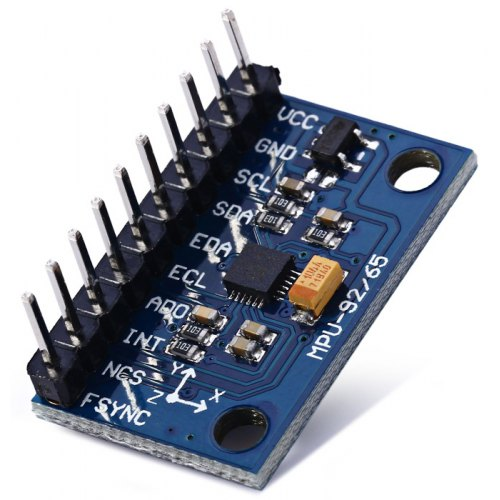
\includegraphics[scale=0.25]{MPU9250.png}
\\

\fontsize{5pt}{6pt}\selectfont https://github.com/Intelligent-Vehicle-Perception/MPU-9250-Sensors-Data-Collect
\end{tabular}
\end{tabular}
\end{frame}

\begin{frame}
\frametitle{RPM Sensor}
\begin{tabular}{cl}
\begin{tabular}{l}
\onslide<1>{\checkmark \ Code working}
\\

\onslide<2>{$\thicksim$ Mounted}
\\

\onslide<3>{\xmark \; Tested}
\\

\onslide<4>{\xmark \; Finished}
\end{tabular}
\begin{tabular}{c}
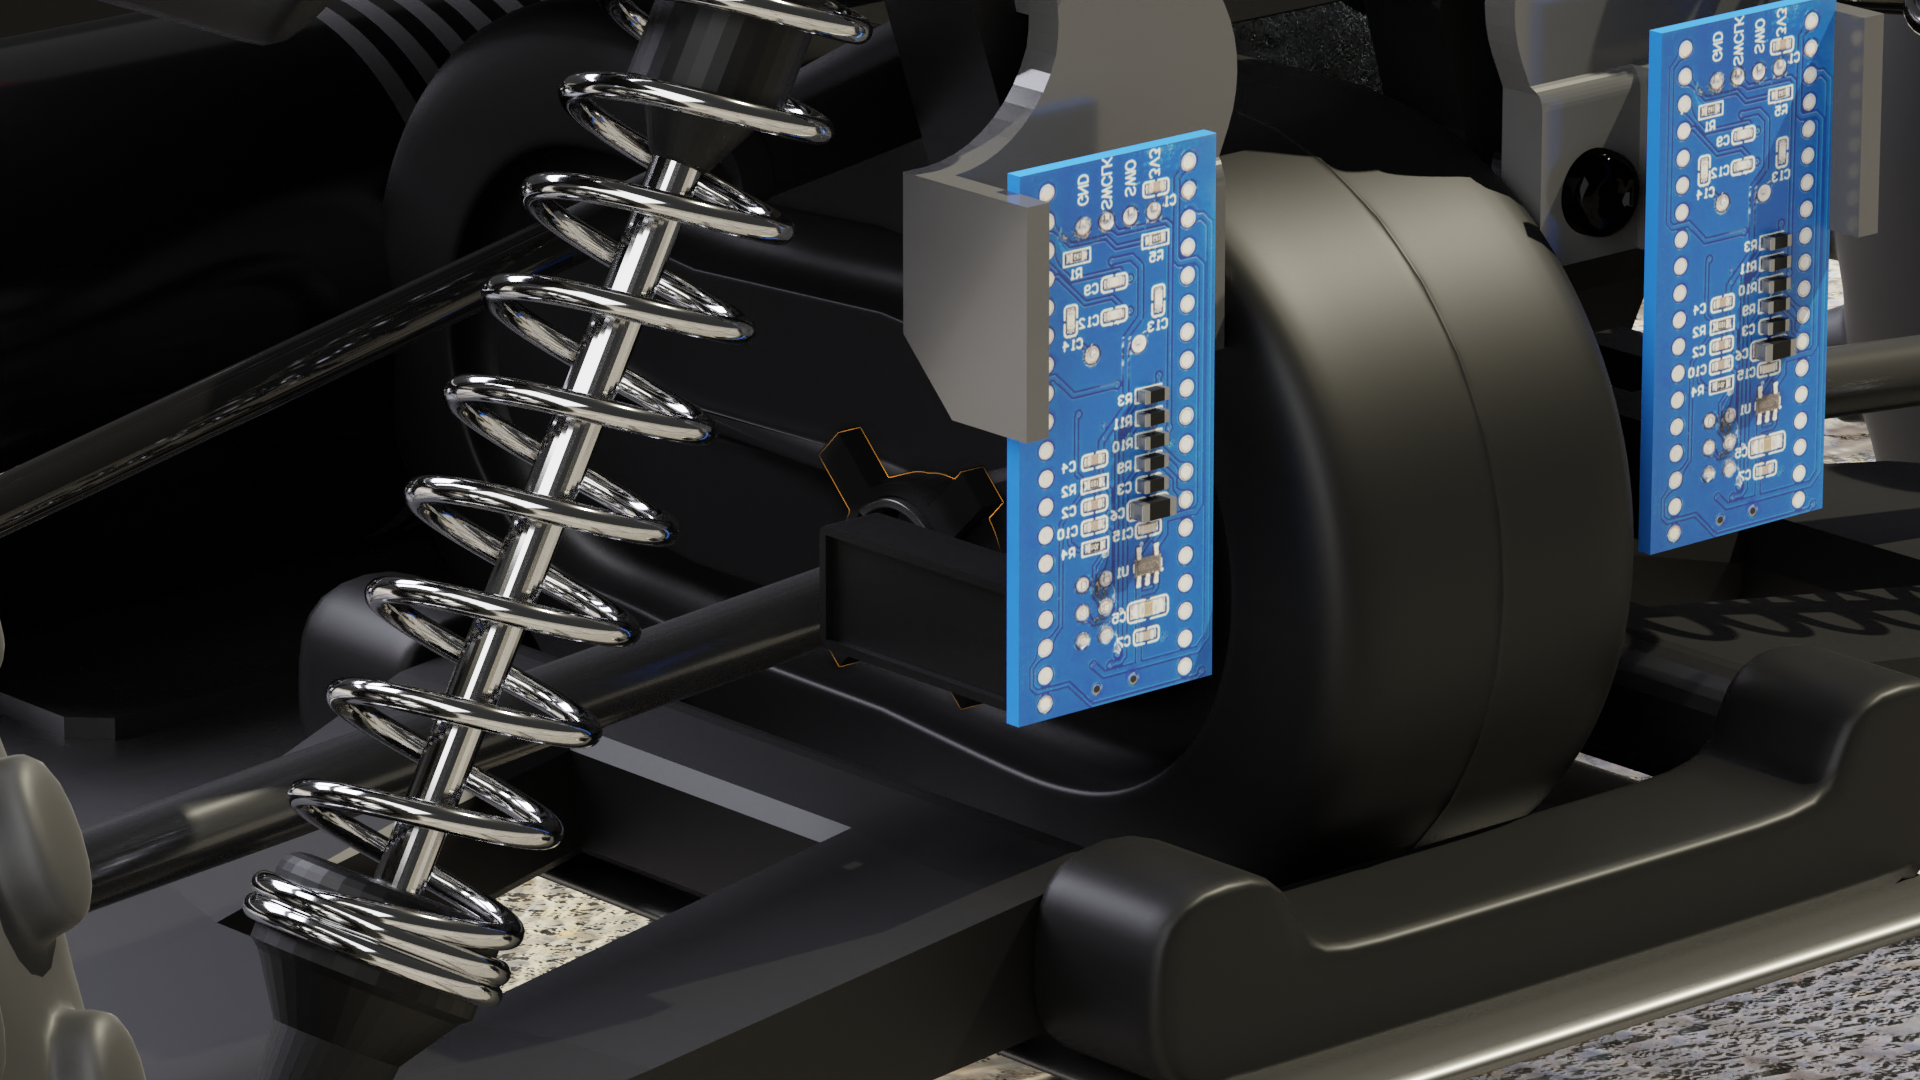
\includegraphics[scale=0.1]{rpm_rear02.png}
\end{tabular}
\end{tabular}
\end{frame}

\begin{frame}
\frametitle{GPS}
\begin{tabular}{cl}
\begin{tabular}{l}
\onslide<1>{\checkmark \ Code working}
\\

\onslide<2>{\xmark \; Mounted}
\\

\onslide<3>{\checkmark \ Tested}
\\

\onslide<4>{\xmark \; Finished}
\end{tabular}
\begin{tabular}{c}
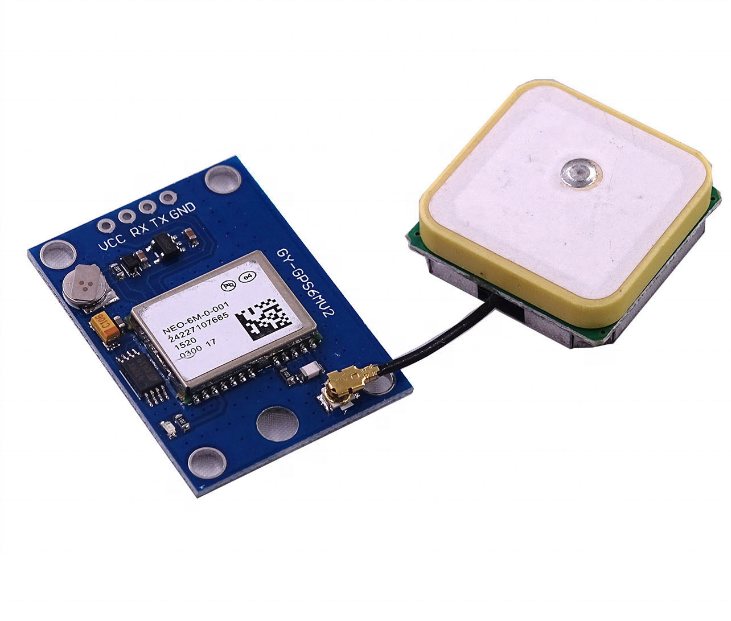
\includegraphics[scale=0.18]{GPS.png}
\\

{\tiny https://nettigo.eu/products/neo6mv2-gps-module-with-active-antenna}
\end{tabular}
\end{tabular}
\end{frame}

\begin{frame}
\frametitle{Desktop-App}
\begin{tabular}{cl}
\begin{tabular}{l}
\onslide<1>{\checkmark \ Base Program}
\\

\onslide<2>{\checkmark \ Table View}
\\

\onslide<3>{$\thicksim$ Plot View}
\\

\onslide<4,5>{\checkmark \ Map View}
\end{tabular}
\begin{tabular}{c}
\only<1>{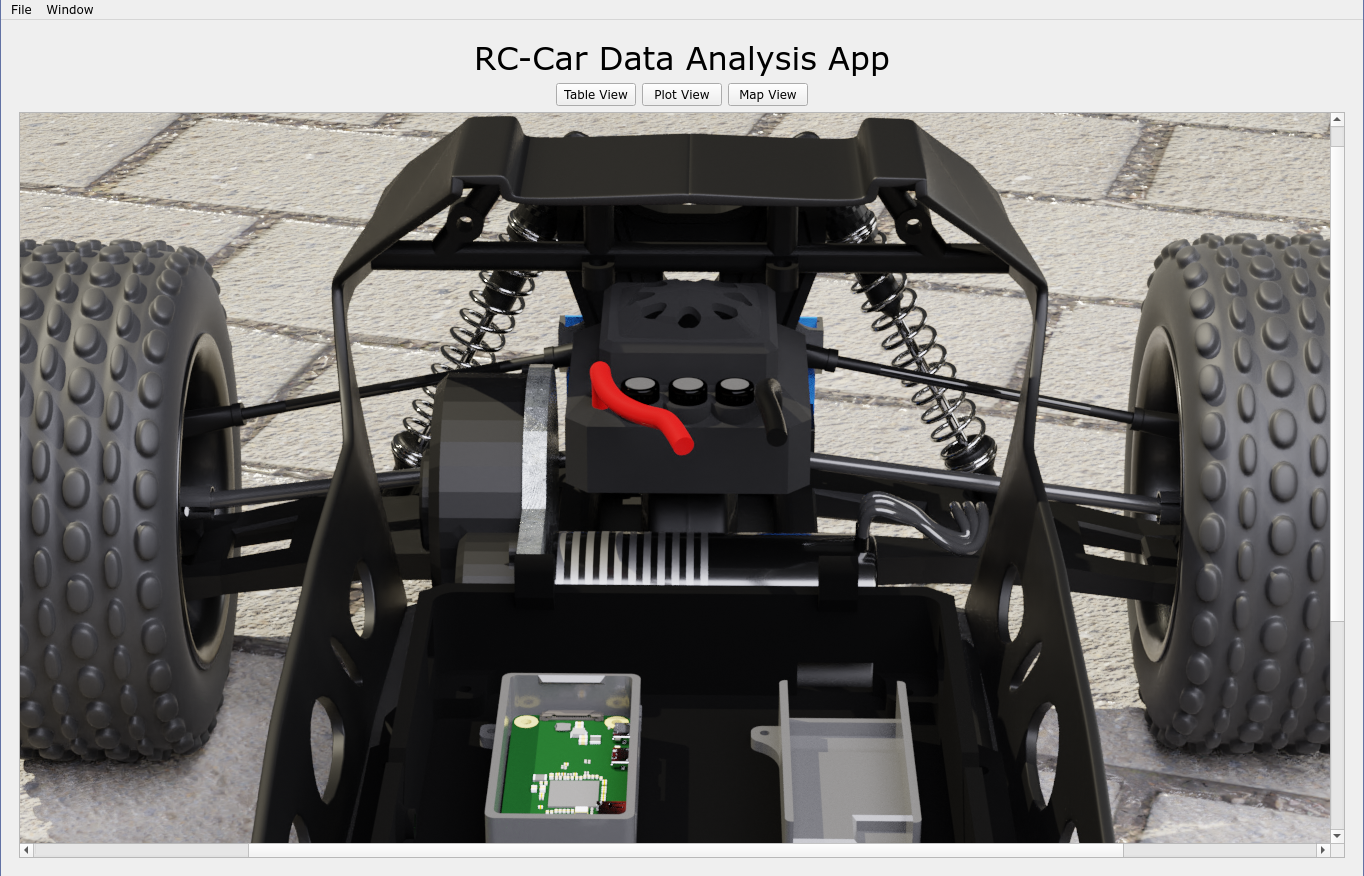
\includegraphics[scale=0.18]{OverView.png}}\only<2>{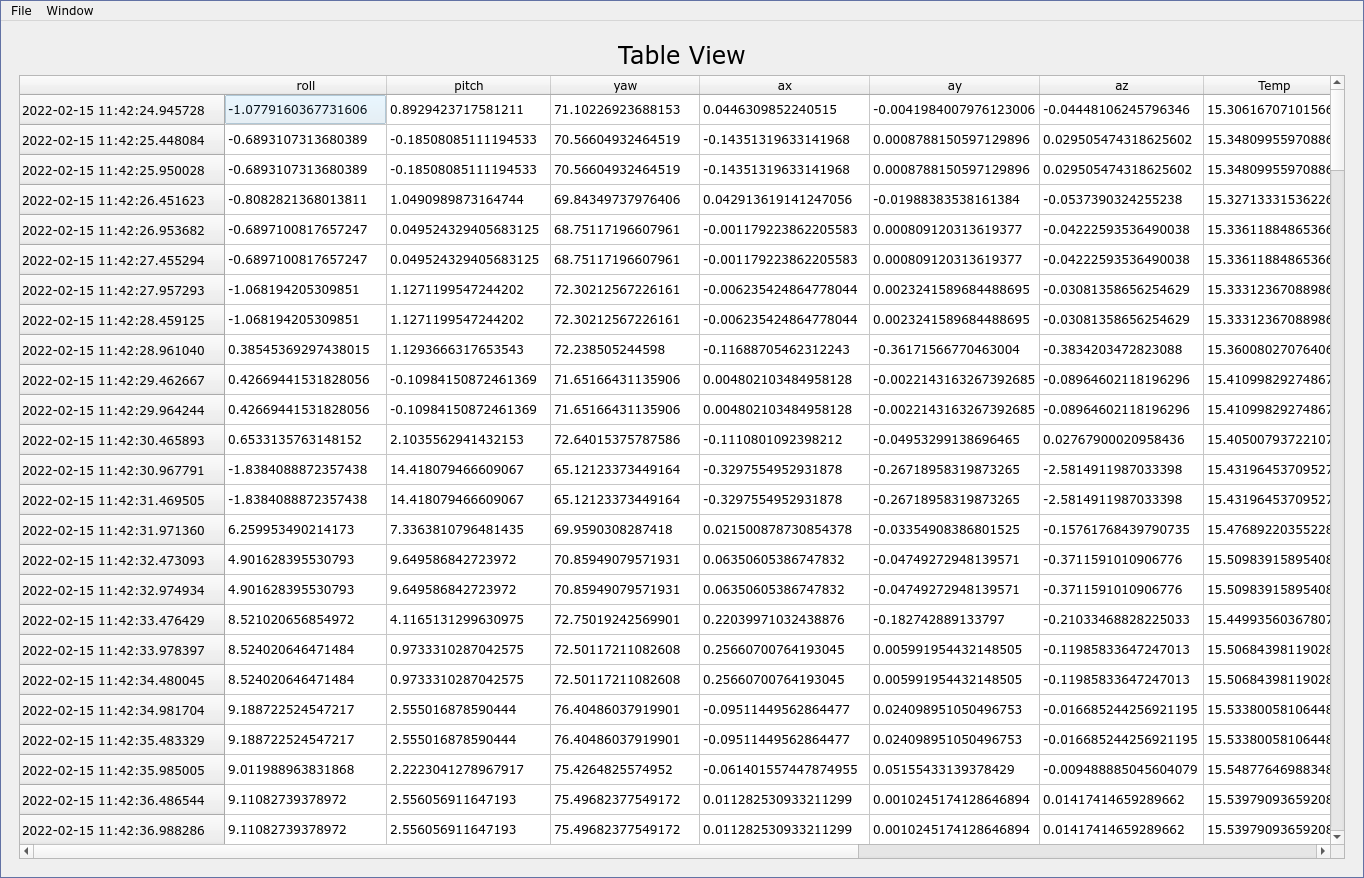
\includegraphics[scale=0.18]{TableView.png}}\only<3>{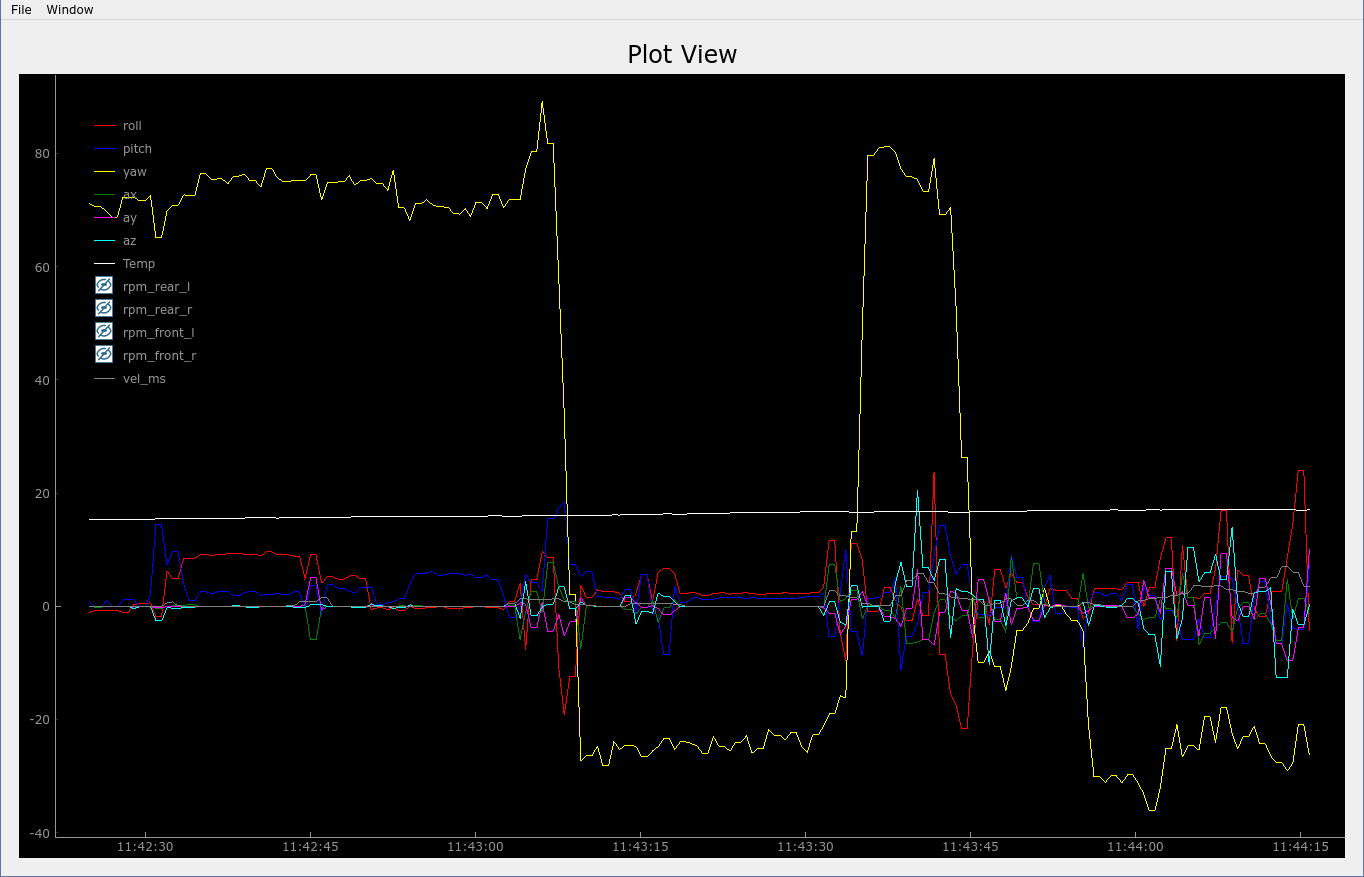
\includegraphics[scale=0.18]{PlotView.png}}\only<4>{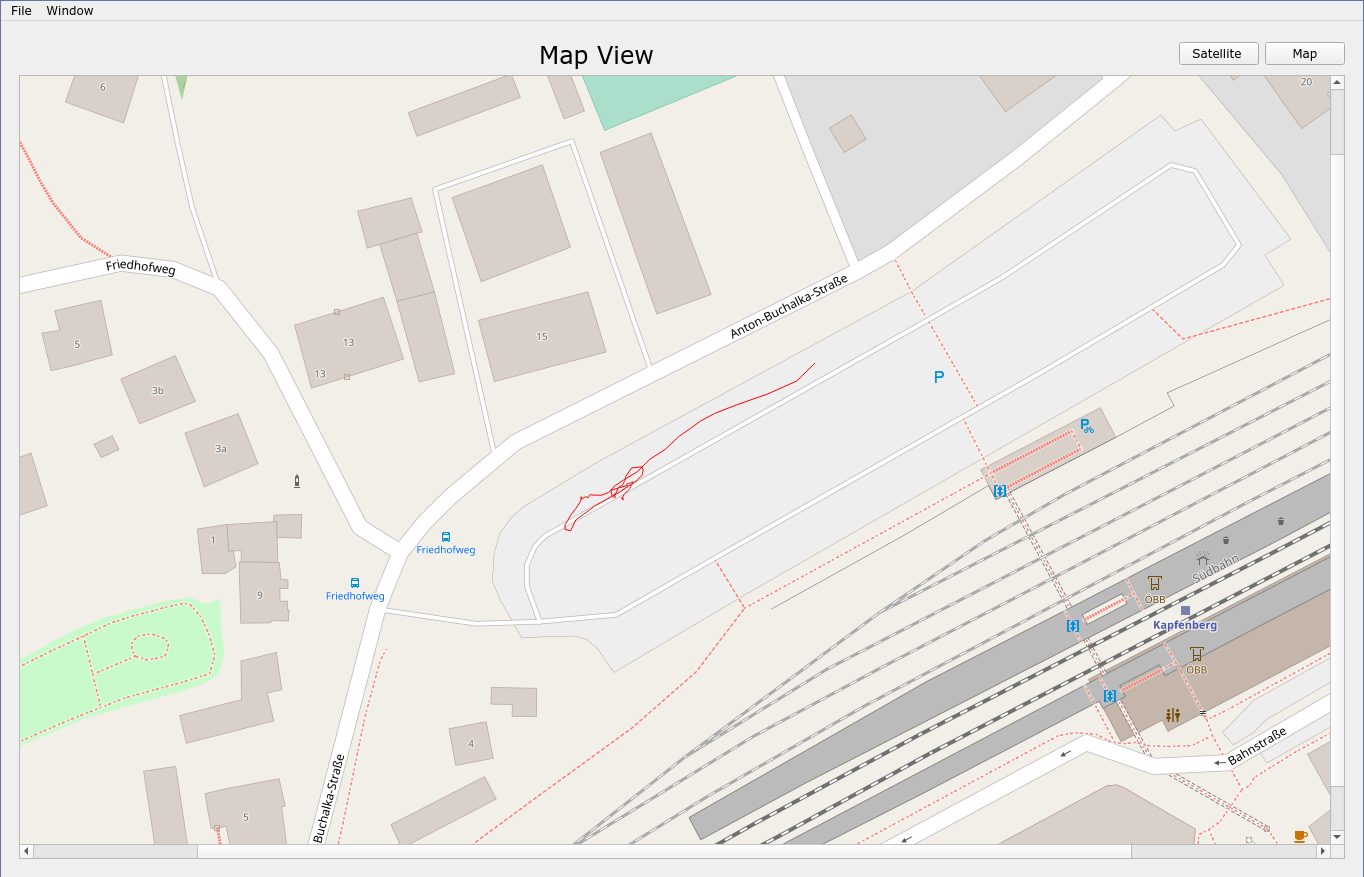
\includegraphics[scale=0.18]{MapView.png}}\only<5>{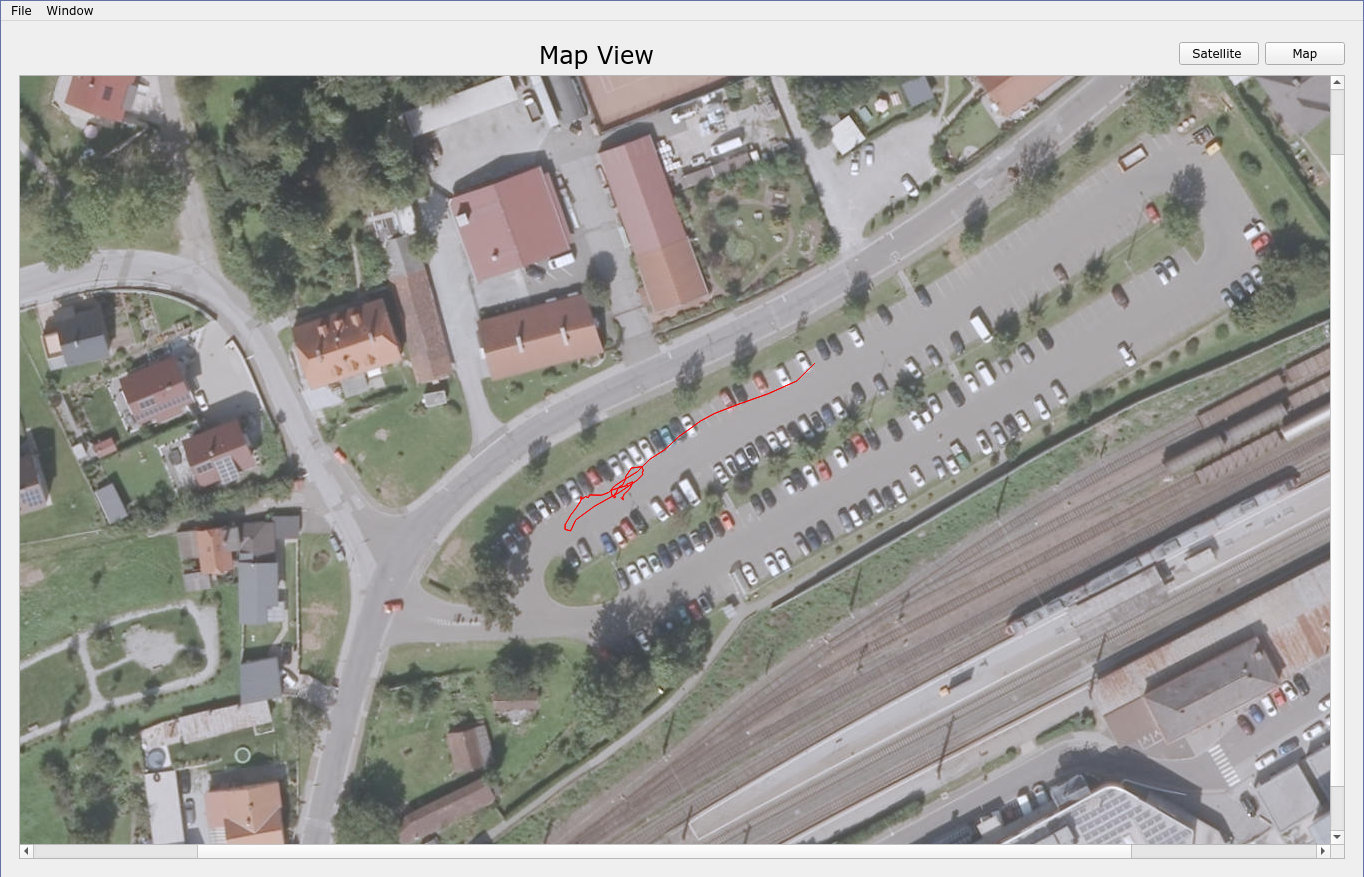
\includegraphics[scale=0.18]{MapViewSatellite.png}}
\end{tabular}
\end{tabular}
\end{frame}

\begin{frame}
\frametitle{Goodies}
\begin{tabular}{cl}
\begin{tabular}{l}
\onslide<1>{\checkmark \ USB Data Transfer Mode}
\\

\onslide<2>{\checkmark \ Status LED}
\\

\onslide<3>{\checkmark \ Voltage Display}
\\

\onslide<4>{$\thicksim$ 3D-Model}
\end{tabular}
\begin{tabular}{c}
\only<2>{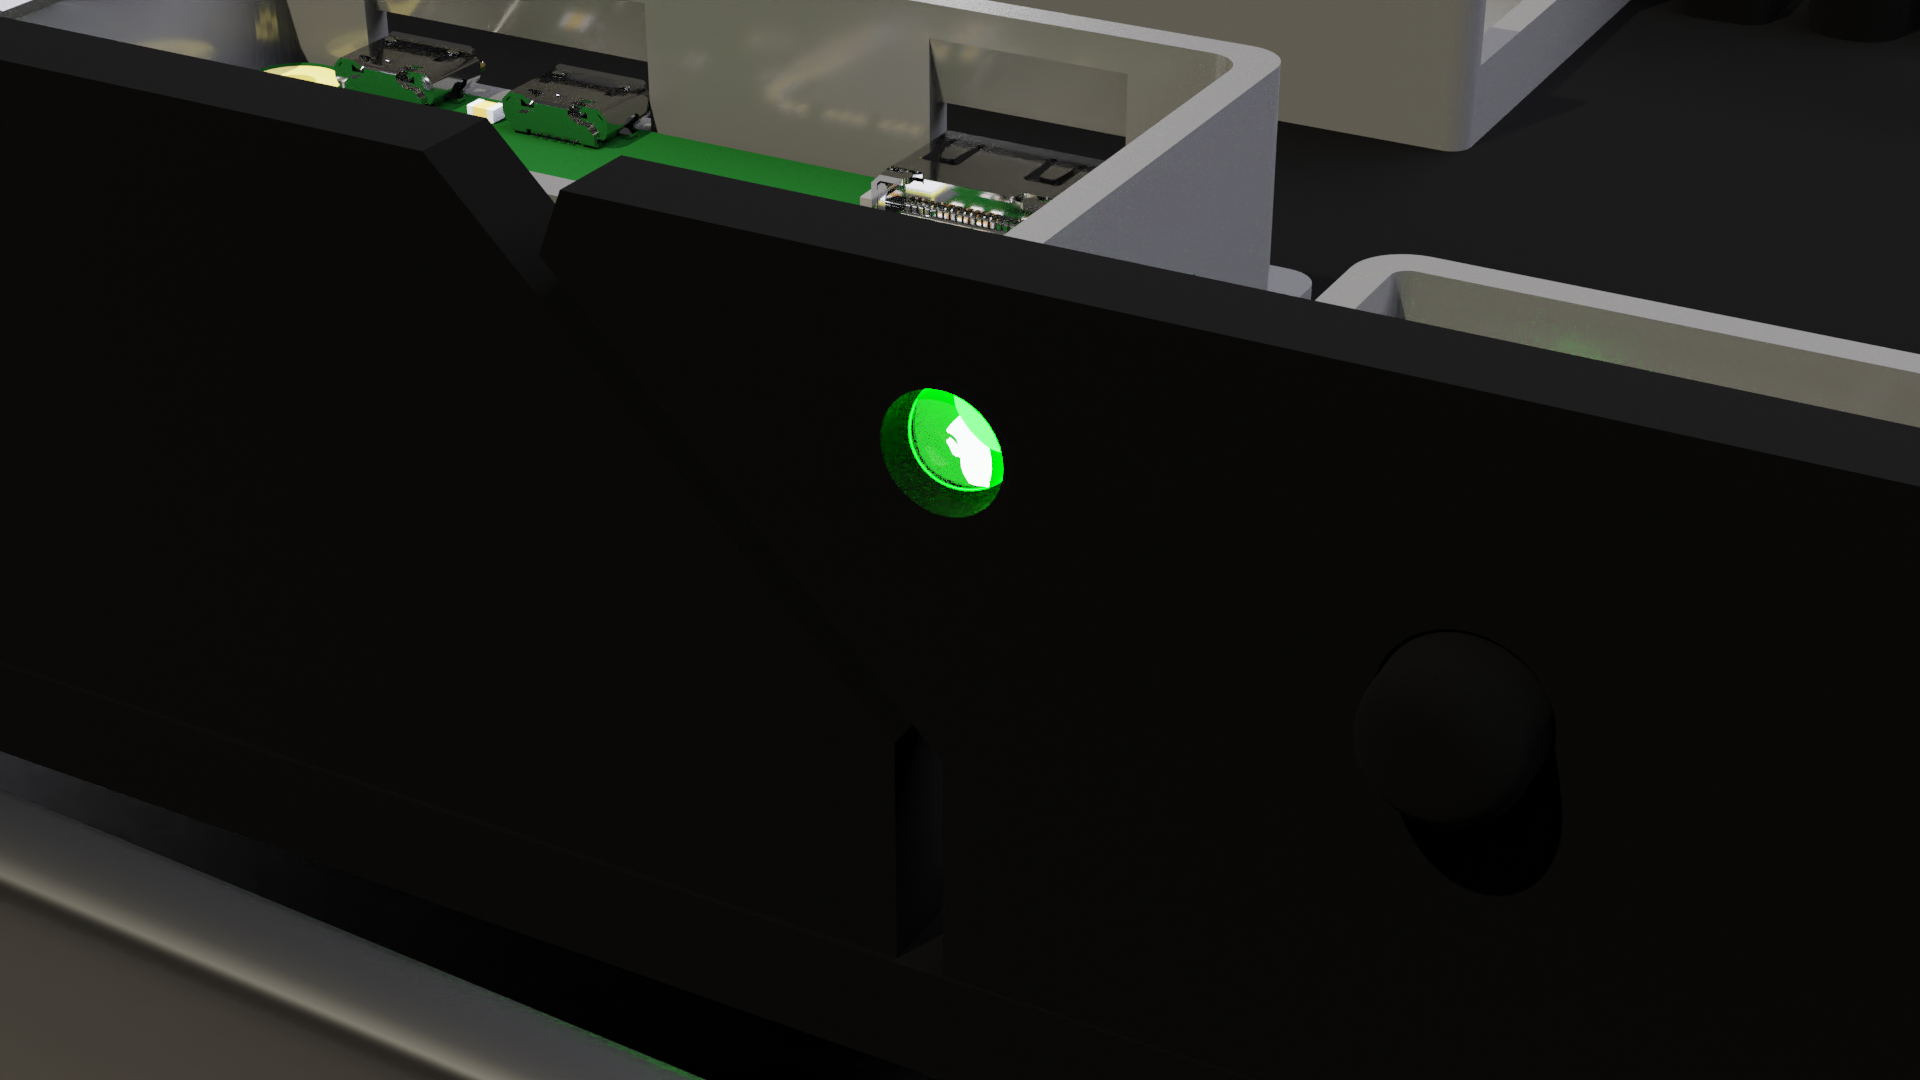
\includegraphics[scale=0.07]{LED.png}}
\only<3>{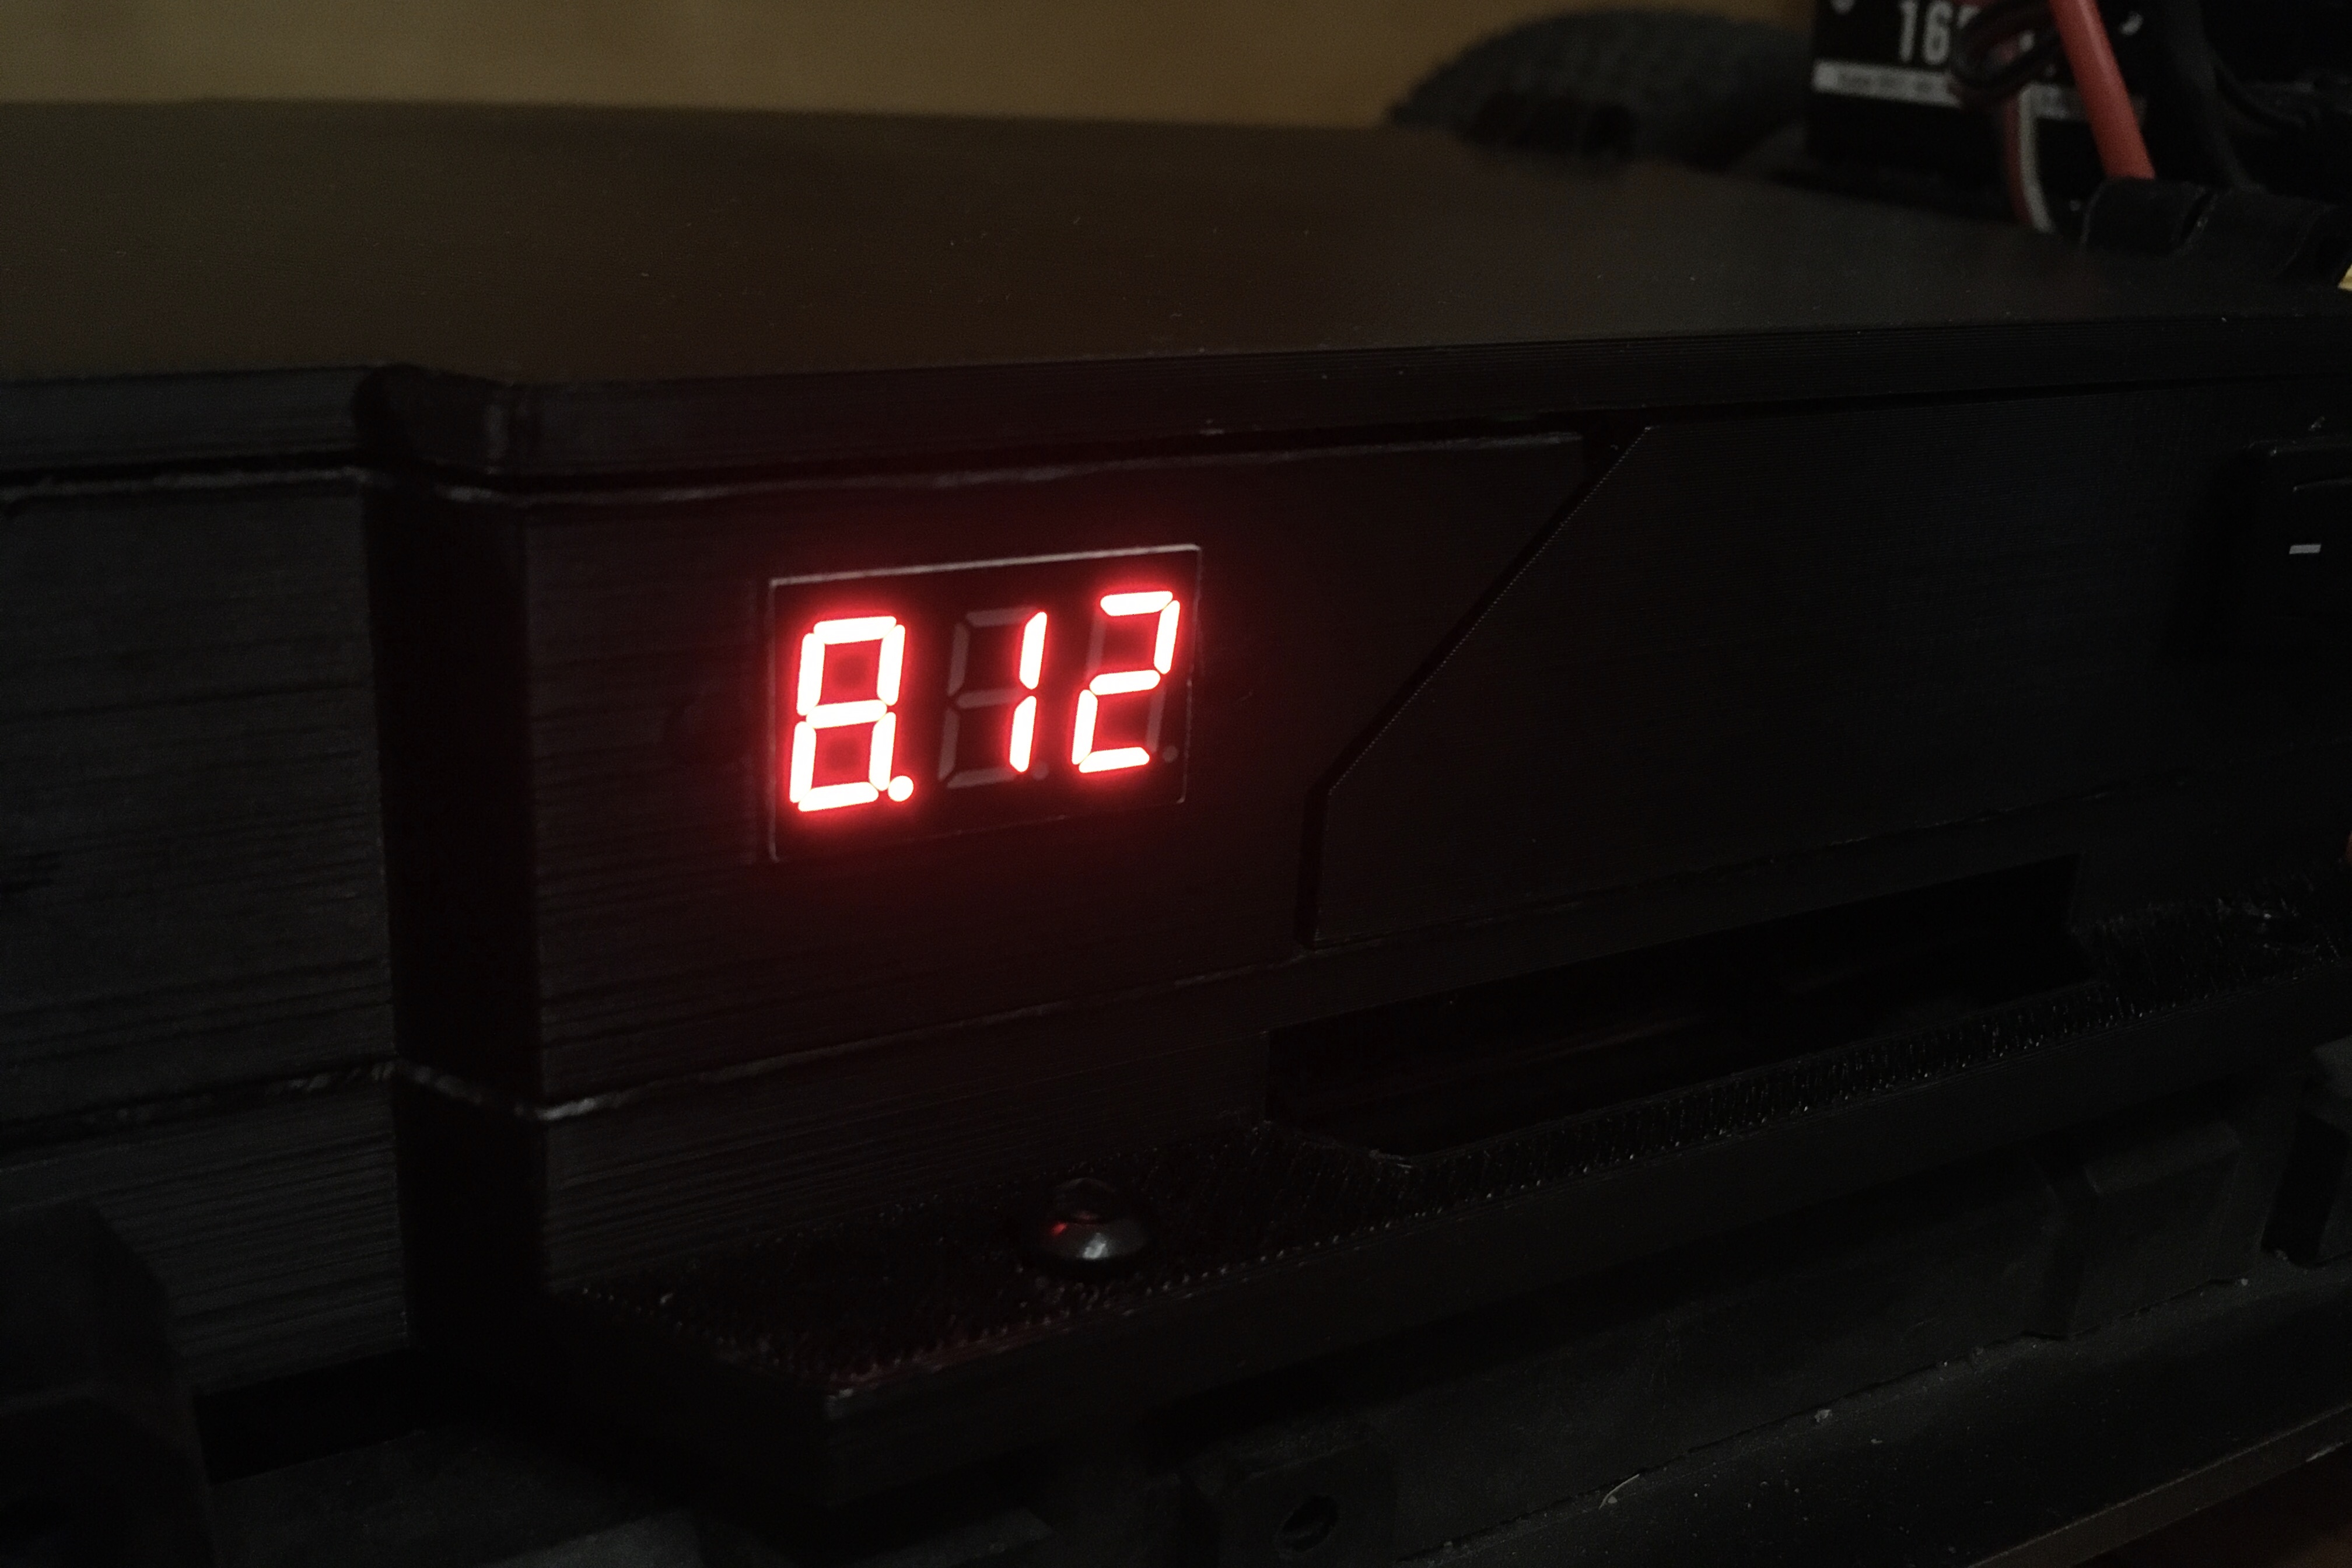
\includegraphics[scale=0.03]{VoltageDisplay.jpg}}
\end{tabular}
\end{tabular}
\end{frame}

\section{Challenges}
\begin{frame}
\frametitle{IMU}
\onslide<1>{Readings incorrect}
\\

\onslide<2>{Earth Acceleration included}
\begin{center}
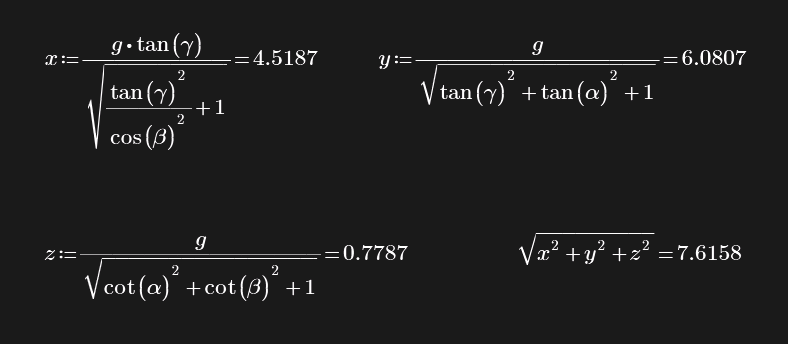
\includegraphics[scale=0.4]{IMUCalc.png}
\end{center}
\end{frame}

\begin{frame}
\frametitle{RPM Sensor}
\onslide<1>{Steering Movement}
\newline
\onslide<2>{Suspension Movement}
\newline
\onslide<3>{Environment Influences}
\end{frame}

\section{Future}
\begin{frame}
\frametitle{Future}
\onslide<1>{Everything mentioned}
\newline
\onslide<2>{Bringing everything to paper}
\end{frame}
\end{document}